\section{Materials and Methods}
\label{ch:methods}

\subsection{Introduction}
\label{sec:m_intro}

This chapter describes the development of the tomato ripening detection and sorting system. The research consists of two main parts: a computer vision component (image collection, model training, and testing) and an engineering component (fabrication of the conveyor belt, electronics, and software). Together, they form a conveyor prototype that detects a tomato on a moving belt, classifies its ripening stage or defect condition, estimates its remaining shelf life, and diverts it into the appropriate output bin.

This chapter is organized chronologically based on the research phases: materials, dataset preparation, model development, real-time detection, hardware and software development, integration, shelf-life observation, and system evaluation. Results are reported in Chapter~\ref{ch:results}; raw data and full component specifications are provided in the appendices.

\subsection{Overall Research Methodology}
\label{sec:m_overall}

This allowed for revisions to the dataset, annotation rules, and AI model whenever evaluations identified issues. The sequential stages were: problem definition; sample collection and image acquisition; dataset preparation, annotation, and splitting; preprocessing and augmentation; model training and testing; dataset correction and retraining; hardware design and fabrication; software development; hardware and software integration; real-time detection and sorting; and system testing. This workflow, including the feedback correction loop, is illustrated in Figure~\ref{fig:methodology}.

\begin{figure}[H]
\centering
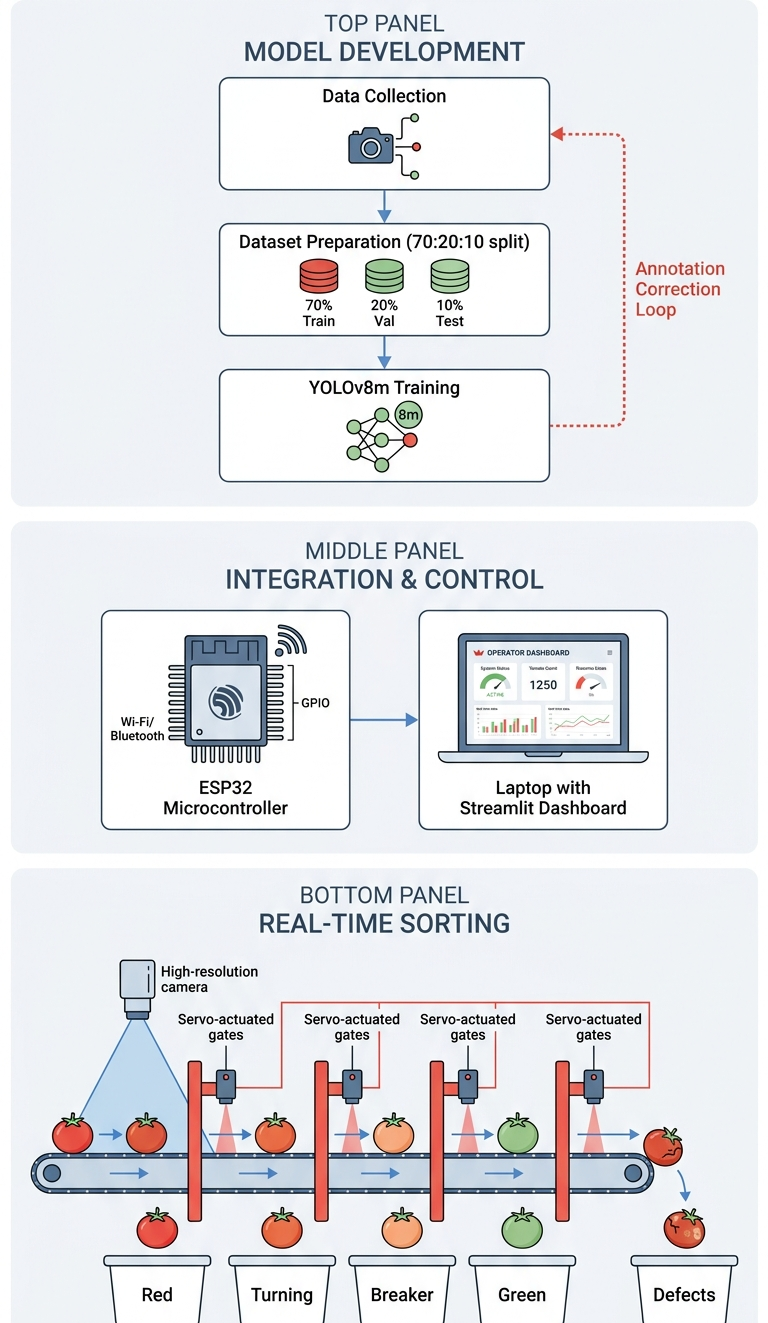
\includegraphics[width=0.5\linewidth]{figures/overallmetho.png}
\caption{Overall research methodology}
\label{fig:methodology}
\end{figure}

\subsection{Research Materials}
\label{sec:m_materials}

\subsubsection{Tomato Samples}
\label{sec:m_samples}

Padma variety tomatoes were acquired from a commercial collecting center in Bandarawela, Badulla District, which receives fruit from multiple regional farms. Sourcing from a multi-farm center rather than a single farm ensures natural variation in size, texture, maturity, and handling damage. Fruits were visually sorted during capture into the five categories defined in Section~\ref{sec:m_classes}. The materials used are listed in Table~\ref{tab:materials}.

\begin{table}[H]
\caption{Materials and samples used in the research}
\label{tab:materials}
\centering
\begin{tabularx}{\textwidth}{p{3.1cm} X p{2.7cm}}
\toprule
\textbf{Material} & \textbf{Description} & \textbf{Purpose} \\
\midrule
Padma tomato fruit &
Fresh fruit at four ripening stages, and fruit with visible cracking, bruising or rot, from a commercial collecting centre, Bandarawela &
Image dataset, shelf-life observation and conveyor testing \\
\addlinespace
Publicly sourced defect images &
Third-party defect images used in an earlier dataset version, captured under uncontrolled backgrounds and lighting &
Removed during quality control (Section~\ref{sec:annotation_qc}) \\
\bottomrule
\end{tabularx}
\end{table}

\subsubsection{Hardware Components}
\label{sec:m_hardware}

The prototype consists of a conveyor belt equipped with a fixed overhead camera and four servo-actuated sorting gates. Its primary components are detailed in Table~\ref{tab:hardware}; the complete pin assignment and wiring diagrams are provided in \hyperref[app:C]{Appendix~C}.


\begin{table}[H]
\caption{Principal hardware components of the conveyor sorting prototype}
\label{tab:hardware}
\centering
\begin{tabularx}{\textwidth}{>{\raggedright\arraybackslash}p{3.5cm} >{\raggedright\arraybackslash}X >{\raggedright\arraybackslash}p{1.5cm}}
\toprule
\textbf{Component} & \textbf{Model / specification} & \textbf{Qty} \\
\midrule
Microcontroller & ESP32 development board (DOIT DEVKIT V1); runs the sorting firmware & 1 \\
Drive motor & NEMA 23 stepper motor & 1 \\
Motor driver & DM542 step-and-direction driver & 1 \\
Power supplies & 24\,V 5\,A driver rail; 12\,V 2\,A logic rail & 1 each \\
Gate actuators & MG995 servo with printed diverter blade, one per ripening class & 4 \\
Presence sensors & Infrared reflective sensor, one at each gate & 4 \\
Power transmission & Motor pulley, roller pulley and timing belt (3:1 reduction) & 1 set \\
Frame and mounts & 25\,mm box-section frame, bearing assemblies, printed brackets, adjustable camera mount & 1 set \\
Speed control & Potentiometer read by the microcontroller & 1 \\
Camera & \acrshort{USB} webcam, 960\,$\times$\,720 pixels, 30~\acrshort{FPS} & 1 \\
Host computer & Workstation with NVIDIA GeForce RTX 3070 Ti, 8{,}192~\acrshort{MiB} \acrshort{VRAM} & 1 \\
\bottomrule
\end{tabularx}
\end{table}





\subsubsection{Software and Technologies}
\label{sec:m_software}

The software environment is listed in Table~\ref{tab:software}.

\begin{table}[H]
\caption{Software, frameworks and libraries used in the research}
\label{tab:software}
\centering
\begin{tabularx}{\textwidth}{>{\raggedright\arraybackslash}p{4.5cm} >{\raggedright\arraybackslash}X}
\toprule
\textbf{Software} & \textbf{Purpose} \\
\midrule
Python, PyTorch/torchvision, Ultralytics (YOLOv8) & Model training, validation and inference \\
OpenCV & Camera capture, frame processing, box rendering \\
Albumentations & Offline bounding-box-aware augmentation \\
Streamlit and Plotly & Operator dashboard and charts \\
SQLite & Local detection and indicator database \\
Roboflow & Annotation and versioned dataset export \\
PlatformIO, Arduino framework, ESP32Servo & Firmware build, upload and servo control \\
SolidWorks and Onshape & Three-dimensional design of the prototype \\
\bottomrule
\end{tabularx}
\end{table}




\subsection{Sampling Method and Sample Collection}
\label{sec:m_sampling}

Images were collected using purposive sampling rather than random sampling: fruits were deliberately photographed across all five target categories to ensure that the less common defect condition was adequately represented \citep{etikan2016}.

Data collection commenced in January 2026. All dataset images were captured with the fruit placed against a white background inside a lightbox under \acrshort{LED} illumination. This maintained consistent background and lighting conditions across all sessions and classes. This consistency was crucial: as explained in Section~\ref{sec:annotation_qc}, images captured under variable lighting conditions caused the model to learn the background lighting instead of the fruit characteristics.

\subsection{Image Acquisition}
\label{sec:m_acquisition}

The real-time deployment setup utilizes a different camera configuration than the dataset capture process. For real-time inference, the system uses a \acrshort{USB} webcam mounted above the conveyor belt, operating at 960\,$\times$\,720 pixels and 30~\acrshort{FPS}. Upon initialization, the camera's automatic exposure and white balance are allowed approximately 1.5~seconds to stabilize before any frame is sent to the model. Frames captured during this initial period can exhibit severe color distortions that may alter the predicted class, and are therefore discarded.

\begin{figure}[H]
\centering
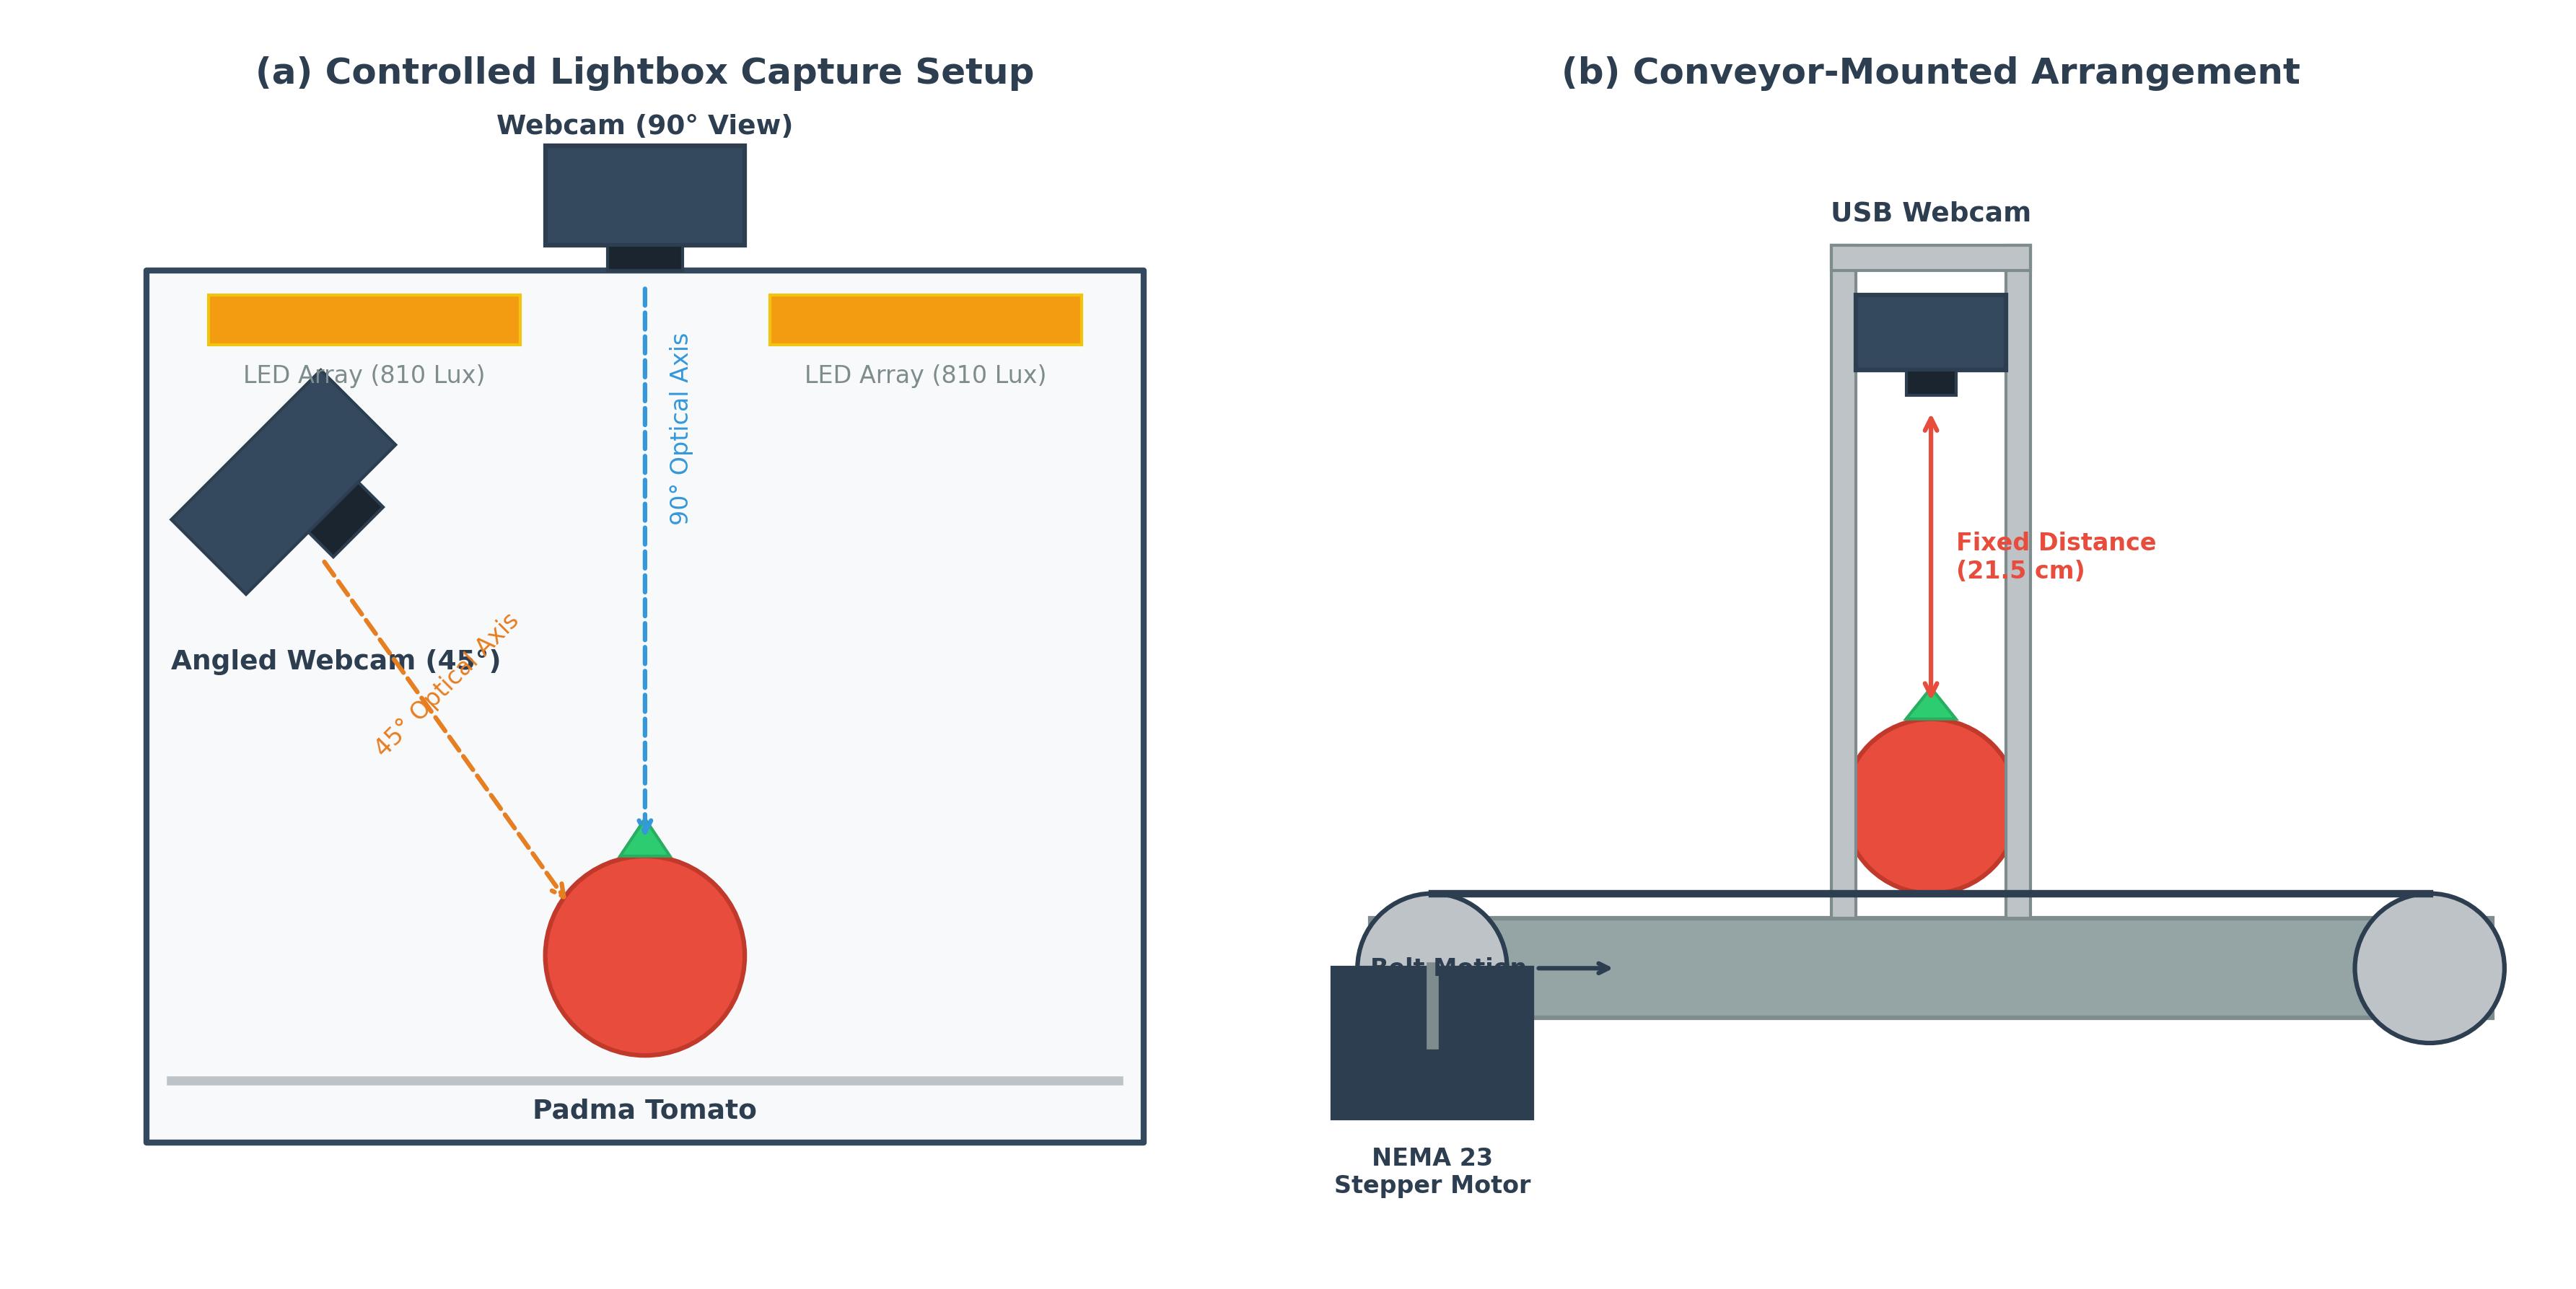
\includegraphics[width=0.9\linewidth]{figures/lightbox.png}
\caption{Image acquisition setup for dataset capture and the conveyor mounted camera arrangement}
\label{fig:acquisition}
\end{figure}

\subsection{Dataset Description}
\label{sec:m_dataset}

The dataset was compiled and versioned using Roboflow \citep{dwyer2024} and exported in the YOLOv8 label format. Its composition is detailed in Table~\ref{tab:dataset}, and the per-class instance counts are provided in Table~\ref{tab:instances}. Instance counts exceed image counts because a single image may contain multiple fruits. The images added to augment the defect class (Section~\ref{sec:m_preprocessing}) are listed separately to prevent the mixing of synthetic and captured data in the metrics.

\begin{table}[H]
\caption{Composition of the dataset used for model development}
\label{tab:dataset}
\centering
\begin{tabularx}{\textwidth}{p{6.2cm} X}
\toprule
\textbf{Property} & \textbf{Value} \\
\midrule
Number of classes & 5 (breaker, defect, green, red, turning) \\
Training images & 5{,}498 captured, plus 668 offline-augmented defect images \\
Validation images & 1{,}574 \\
Test images (held out) & 777 \\
Total distinct captured images & 7{,}849 \\
Annotation format & YOLO normalised bounding box: class index, $x$ centre, $y$ centre, width, height \\
Model input resolution & 640\,$\times$\,640 pixels after resizing \\
\bottomrule
\end{tabularx}
\end{table}

\begin{table}[H]
\caption{Per class annotated object instance counts by dataset split}
\label{tab:instances}
\centering
\begin{tabular}{lrrrrr}
\toprule
\textbf{Class} & \textbf{Train} & \textbf{Train} & \textbf{Validation} & \textbf{Test} & \textbf{Total} \\
 & \textbf{(captured)} & \textbf{(augmented)} & & & \\
\midrule
breaker & 1{,}137 & 0   & 326 & 191 & 1{,}654 \\
defect  & 448   & 896 & 137 & 66  & 1{,}547 \\
green   & 1{,}380 & 0   & 429 & 191 & 2{,}000 \\
red     & 1{,}434 & 0   & 395 & 190 & 2{,}019 \\
turning & 1{,}138 & 0   & 309 & 149 & 1{,}596 \\
\midrule
\textbf{Total} & \textbf{5{,}537} & \textbf{896} & \textbf{1{,}596} & \textbf{787} & \textbf{8{,}816} \\
\bottomrule
\end{tabular}
\end{table}

The defect class contains only 66 test instances, compared to 149--191 for each ripening class. Consequently, it is treated with increased statistical caution in the evaluation approach detailed in Section~\ref{sec:m_evaluation}.

\begin{figure}[H]
\centering
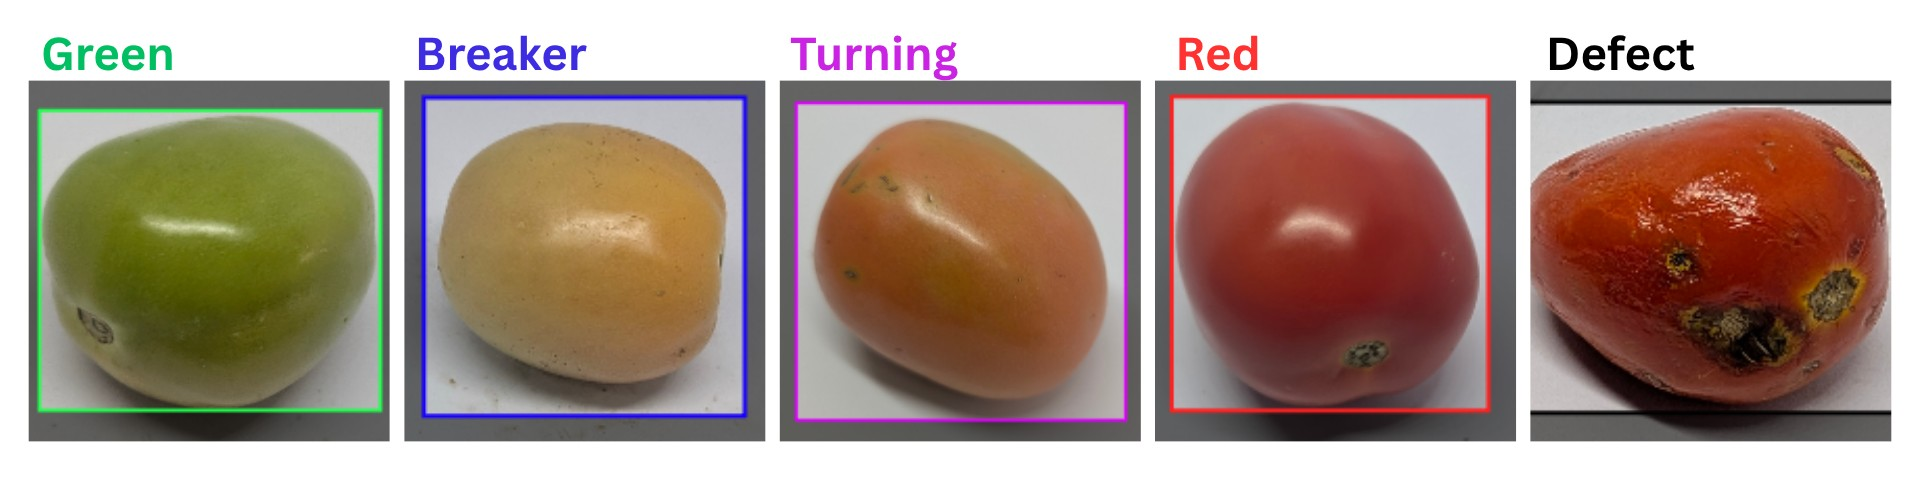
\includegraphics[width=0.9\linewidth]{figures/bounding.jpeg}
\caption{Representative sample images for each of the five target classes}
\label{fig:classes}
\end{figure}

\subsection{Ripening Stage Classification Criteria}
\label{sec:m_classes}

Five classes were established: four ripening stages and one defect class. Defect is treated as a separate class rather than an attribute of a ripening stage, because damaged fruit is handled similarly regardless of its color.

The four ripening stages were defined by merging adjacent pairs of the six standard \acrshort{USDA} maturity stages \citep{usda1991}, aligning with the methodology used by \citet{abekoon2024} for this tomato variety. The four classes correspond directly to the four sorting gates. Furthermore, the two narrowest standard bands occur where a camera has the most difficulty estimating the red surface percentage. Merging these bands creates broader boundaries that the model can reliably distinguish on a moving conveyor belt. This correspondence is outlined in Table~\ref{tab:merge}, and the resulting criteria are shown in Table~\ref{tab:ripeness}.

\begin{table}[H]
\caption{Correspondence between the six standard maturity stages and the four operational classes used in this research}
\label{tab:merge}
\centering
\begin{tabular}{llll}
\toprule
\textbf{Standard stage} & \textbf{Standard red surface} & \textbf{Operational class} & \textbf{Operational red surface} \\
\midrule
Green      & 0\,\%      & Green   & 0\,\% \\
\midrule
Breaker    & $\leq$ 10\,\%   & \multirow{2}{*}{Breaker} & \multirow{2}{*}{$<$ 30\,\%} \\
Turning    & 10--30\,\% &         & \\
\midrule
Pink       & 30--60\,\% & \multirow{2}{*}{Turning} & \multirow{2}{*}{30--80\,\%} \\
Light red  & 60--90\,\% &         & \\
\midrule
Red        & $>$ 90\,\%  & Red     & $>$ 80\,\% \\
\bottomrule
\end{tabular}

\vspace{2mm}
{\footnotesize Standard stages and boundaries from \citet{usda1991}. The operational upper boundary of the turning class is set at 80\,\% rather than 90\,\% so that fully coloured fruit falls into the red class under belt lighting.}
\end{table}

\begin{table}[H]
\caption{Ripening stage and quality classes used in this research}
\label{tab:ripeness}
\centering
\begin{tabularx}{\textwidth}{p{1.9cm} p{3.3cm} X}
\toprule
\textbf{Class} & \textbf{Stage} & \textbf{Identification characteristics} \\
\midrule
Green   & Unripe (Stage 1)             & Entirely green skin, no red or orange colouration \\
Breaker & Onset of ripening (Stage 2)  & Green-to-yellow transition, less than 30\,\% red or pink \\
Turning & Mid ripening (Stage 3)       & 30--80\,\% of the surface red, mixed green/orange/red patches \\
Red     & Fully ripe (Stage 4)         & More than 80\,\% of the surface red, uniform ripe colouration \\
Defect  & Rejected quality             & Visible cracking, bruising or rot; can occur at any stage, receives no ripening label \\
\bottomrule
\end{tabularx}
\end{table}

\subsection{Image Annotation}
\label{sec:m_annotation}

All images were annotated using Roboflow \citep{dwyer2024} and exported in the YOLOv8 format. In this format, each image includes a corresponding label file containing one line per annotated fruit: a class index followed by the bounding box's normalized position and dimensions.

Every fruit visible in an image was assigned an individual bounding box and a single class label. For the defect class, the bounding box encompasses the entire fruit, rather than just the blemished area, and is labeled as defective regardless of the fruit's underlying ripeness color. Maintaining a consistent bounding box style across all classes is essential, as the model learns the typical spatial dimensions for each class in addition to its visual features.

\begin{figure}[H]
\centering
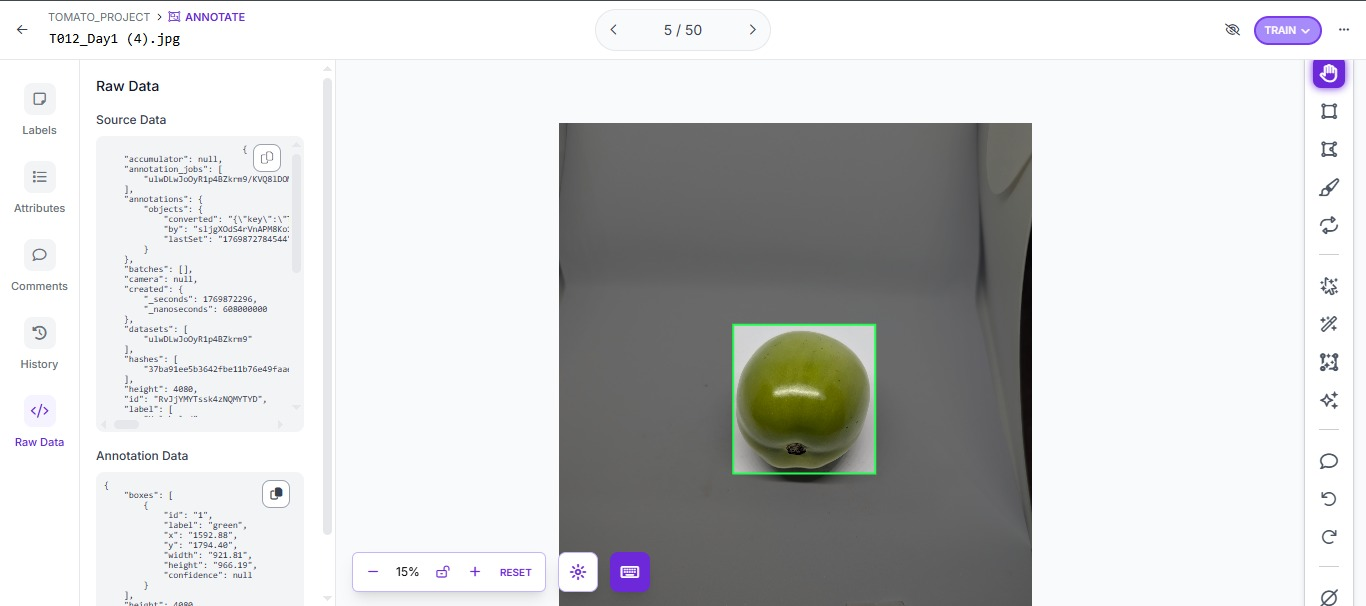
\includegraphics[width=0.9\linewidth]{figures/Annotate.jpeg}
\caption{Example of bounding box annotation for a tomato image}
\label{fig:annotation}
\end{figure}

\subsubsection{Annotation Quality Control and Correction}
\label{sec:annotation_qc}

The annotation process included a review and correction cycle. Two major corrections influenced the final dataset:

\begin{itemize}
    \item \textbf{Inconsistent box style.} Defect images sourced from a public dataset were originally annotated with bounding boxes around only the blemished areas, whereas the newly captured project images annotated the entire fruit. Every such image was re-annotated using the whole-fruit style to ensure geometric consistency across all five classes. 
    \item \textbf{Lighting acting as a false class cue.} Even after standardizing the bounding box style, live camera tests revealed that healthy breaker, turning, and red fruits were incorrectly classified as defective. This occurred because most defect images originated from the public dataset, which featured different backgrounds and lighting compared to the other four classes captured inside the lightbox. Consequently, the model incorrectly learned the lighting conditions, rather than the physical damage, as the indicator of a defect. The solution was to remove the mismatched public images, capture and label new defect images under the identical lightbox conditions, and apply the offline augmentation described in Section~\ref{sec:m_preprocessing} to compensate for the reduced number of authentic defect photos. The dataset presented in Section~\ref{sec:m_dataset} represents this corrected version.
\end{itemize}

The detailed annotation procedure is provided in \hyperref[app:A]{Appendix~A}.

\subsection{Image Preprocessing and Augmentation}
\label{sec:m_preprocessing}

All images were resized to 640\,$\times$\,640 pixels for both training and inference, which is the standard input resolution for this architecture.During training, images undergo real-time augmentation. Vertical flipping was excluded, as fruit on a conveyor belt is never oriented upside down. This augmentation is standard practice for improving model generalization from limited data \citep{shorten2019}, and was utilized here because real-world conveyor lighting differs from the lightbox conditions used during dataset capture.

Following the corrections outlined in Section~\ref{sec:annotation_qc}, the defect class contained significantly fewer real training images than the ripening classes. Therefore, its training images were supplemented offline using the Albumentations library \citep{buslaev2020}. Transformations including flip, rotation, scale, brightness, and hue changes were applied to generate two augmented copies of each defect training image. These additional images were utilized exclusively for training; the validation and test sets consisted solely of originally captured images.

An automated validation script executes before every training session and halts the process if structural errors are detected. It verifies the class list, confirms the existence of a test split, counts images and instances per class, flags missing or empty label files as well as duplicate images, and identifies any class with unusually small bounding boxes compared to the others. This final check was implemented following the box-style issue discussed above, ensuring that inconsistent box conventions do not enter the training phase unnoticed.

\subsection{Dataset Splitting}
\label{sec:m_splitting}

The dataset was divided into training, validation, and test sets at the time of export, using the proportions detailed in Table~\ref{tab:split} (a standard 70:20:10 split). The training set is used to fit the model parameters. The validation set is evaluated after every epoch to select the optimal model checkpoint. Finally, the test set is used only once, at the conclusion of the study, to measure the final unbiased performance.

\begin{table}[H]
\caption{Dataset split used for model development}
\label{tab:split}
\centering
\begin{tabularx}{\textwidth}{l r r X}
\toprule
\textbf{Subset} & \textbf{Images} & \textbf{Percentage} & \textbf{Role} \\
\midrule
Training   & 5{,}498 & 70.0\,\% & Fitting model parameters; supplemented with 668 augmented defect images \\
Validation & 1{,}574 & 20.1\,\% & Monitoring generalisation, early stopping, checkpoint selection \\
Test       & 777   & 9.9\,\%  & Held out from training; used once for final evaluation \\
\midrule
\textbf{Total} & \textbf{7{,}849} & \textbf{100\,\%} & \\
\bottomrule
\end{tabularx}
\end{table}

\subsection{Model Development}
\label{sec:m_model}

The system employs YOLOv8, an object detection architecture that localizes and classifies objects in a single pass over the image, eliminating the need for a separate region proposal step \citep{redmon2016, terven2023}. The medium-sized YOLOv8m variant was utilized. The model was initialized with publicly released pre-trained weights and subsequently fine-tuned on the project's custom dataset.

This architecture is well-suited for the task: a single camera frame above the conveyor may contain multiple fruits at different ripening stages. The sorting logic requires a bounding box, a class label, and a confidence score for each fruit, and it must process this information fast enough to match the conveyor belt speed. Published literature supports this choice for tomato detection \citep{safira2026}. Furthermore, the medium variant optimally balances accuracy with the memory constraints of the host \acrshort{GPU}. No separate classification step is required post-detection; the sorting decision relies directly on the detector's prediction, which is aggregated across frames as detailed in Section~\ref{sec:m_realtime}.

A second detector (YOLO26m) was also trained using the same dataset. This allowed the chosen architecture to be validated using experimental evidence from this specific project, rather than relying solely on published literature. This comparison is detailed as Experiment~2 in Section~\ref{sec:m_experiments}.

\subsection{Model Training}
\label{sec:m_training}

Training was conducted locally on a workstation equipped with an NVIDIA GeForce RTX 3070 Ti \acrshort{GPU} (8{,}192~\acrshort{MiB} \acrshort{VRAM}). Due to the memory limitations of this GPU, the training script automatically selects an appropriate batch size and verifies available memory before initiating each run. The configuration used is summarized in Table~\ref{tab:training}; the complete configuration file is provided in \hyperref[app:B]{Appendix~B}.

\begin{table}[H]
\caption{Training configuration used for model development}
\label{tab:training}
\centering
\begin{tabularx}{\textwidth}{p{5.4cm} X}
\toprule
\textbf{Parameter} & \textbf{Value} \\
\midrule
Base architecture & YOLOv8m, initialised from pre-trained weights \\
Training data & 5{,}498 captured images and 668 offline-augmented defect images \\
Maximum epochs and early stopping & 150 epochs\\
Batch size and input size & Automatic selection; 640\,$\times$\,640 pixels \\
Initial learning rate & 0.01 \\
Augmentation & Colour jitter; rotation, translation, scale; horizontal flip only; mosaic, mixup and random erasing \\
\bottomrule
\end{tabularx}
\end{table}

The training process consists of five steps: verifying that the framework, hardware device, and memory are prepared; executing the dataset audit described in Section~\ref{sec:m_preprocessing}, which aborts the run if anomalies are detected; training the model using the aforementioned settings while monitoring validation performance after each epoch to save the best checkpoint; applying early stopping when performance ceases to improve, retaining the best checkpoint as the final model; and finally, performing a single evaluation pass of that checkpoint on the held-out test set.

\subsection{Validation and Evaluation Procedure}
\label{sec:m_evaluation}

The validation set was evaluated after every epoch during training to prevent overfitting early, utilizing a fixed stopping rule rather than manual observation. The test set was evaluated only once. Therefore, the results reported in Chapter~\ref{ch:results} represent an unbiased estimate rather than values the model was optimized to achieve.

Performance is measured using standard object detection metrics \citep{padilla2020}: precision (the proportion of correct positive predictions), recall (the proportion of actual target instances successfully identified), an $F_1$ score that balances precision and recall (used to select the deployment confidence threshold), and mean average precision evaluated at a standard overlap threshold (mAP@50) and a stricter threshold that accounts for bounding box accuracy (mAP@50--95). A confusion matrix is also generated to illustrate misclassification trends between classes. As noted in Section~\ref{sec:annotation_qc}, this diagnostic tool identified issues that summary statistics alone did not reveal.

Because the test set is limited in size particularly the defect class, which contains only 66 instances confidence interval is calculated for each reported metric using statistical resampling. 

System-level metrics such as total fruits processed, class distribution, defect ratio, throughput, and average shelf life are aggregated directly from the detection logs.

\subsection{Real Time Detection Process}
\label{sec:m_realtime}

During real-time operation, the system executes the following steps for every frame:

\begin{enumerate}
    \item \textbf{Frame capture.} A live video frame is captured from the webcam at 960\,$\times$\,720 pixels and 30~\acrshort{FPS}.
    \item \textbf{Preprocessing.} The frame is resized to the 640\,$\times$\,640 pixel model input dimension.
    \item \textbf{Inference.} The frame is processed through the trained model at a confidence threshold of 0.45, which represents the optimal balance between precision and recall.
  
    \item \textbf{Tracking and vote accumulation.} A tracking algorithm follows individual fruits across consecutive frames and records a class prediction vote from each frame it appears in. A track terminates after 0.6~seconds without a detection, and requires a minimum of two frames to be considered valid.
    \item \textbf{Classification finalisation.} When tracking concludes, the final class is determined by a confidence-weighted majority vote across all recorded frames. Utilizing multiple frames rather than a single frame makes the classification more robust against sudden fruit rotations or temporary light reflections.
\end{enumerate}

The defect class incorporates an additional strict rule: it is only assigned as the final classification if it receives a clear majority of votes across the tracked frames with consistently high confidence. This is a deliberate operational trade-off: incorrectly rejecting a healthy fruit causes a direct financial loss, whereas allowing a borderline fruit to pass can still be identified in later quality control stages. This rule also provides a secondary safeguard against the lighting confound discussed in Section~\ref{sec:annotation_qc}.

The final class, its confidence score, and its estimated shelf-life value (Section~\ref{sec:m_shelflife}) are then recorded in the database. When the hardware is connected, this data is converted into a sorting command as detailed in Section~\ref{sec:m_integration}.

\begin{figure}[H]
\centering
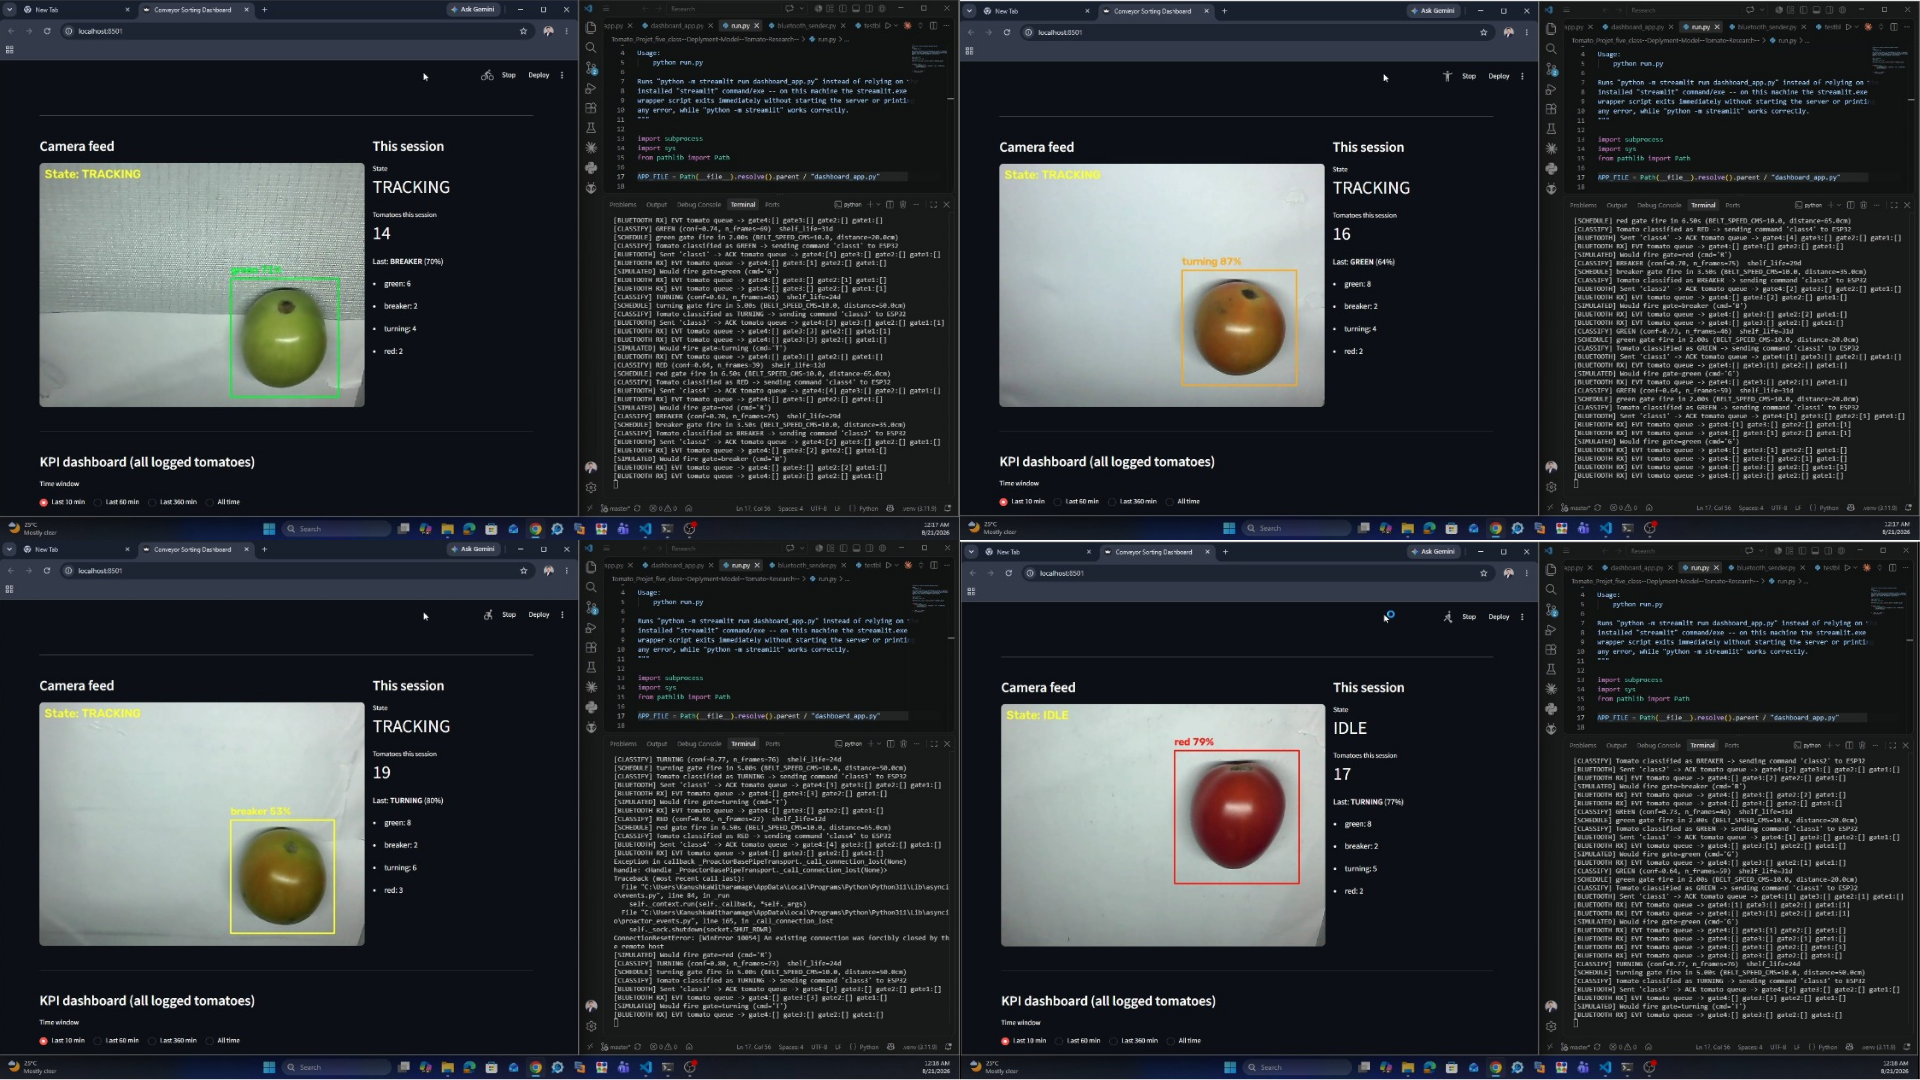
\includegraphics[width=0.9\linewidth]{figures/real time.png}
\caption{Real time tomato detection and classification process}
\label{fig:detection}
\end{figure}

\subsection{Hardware Prototype Development}
\label{sec:m_prototype}

The conveyor frame was constructed using 25\,mm metal box-section bars, based on dimensions verified in a \acrfull{CAD} model. The conveyor belt is driven by a NEMA~23 stepper motor through a 3:1 pulley-and-belt reduction system, supported by bearing assemblies. The motor is controlled via a DM542 driver, with the belt speed regulated by a potentiometer connected to the microcontroller. An adjustable camera mount allows for fine-tuning of the camera position and angle on the assembled structure.

Four infrared sensors and four servo gates are installed, providing one pair for each ripening class. The defect class intentionally lacks a sorting gate: a fruit classified as defective receives no actuation command and travels to the end of the conveyor belt into a single rejection bin.

The physical order of the gates is important for the control logic outlined in Section~\ref{sec:m_integration}: moving downstream from the camera, the gates are arranged as red, turning, breaker, and green. Each gate features an individual sensor positioned immediately before its diverter blade. Furthermore, each gate utilizes dedicated servo and sensor wiring, with the class-to-gate mapping hardcoded into the firmware. The gates rest at 180\textdegree{} and actuate to 110\textdegree{} to divert a fruit, automatically returning to the resting position afterward.

A single ESP32 microcontroller board manages the entire system. It is powered by a 24\,V supply for the motor and a separate 12\,V supply for the logic components. This isolated power design ensures that motor and servo electrical noise does not interfere with the control electronics. The pin assignments and wiring diagrams are provided in \hyperref[app:C]{Appendix~C}.

\begin{figure}[H]
\centering
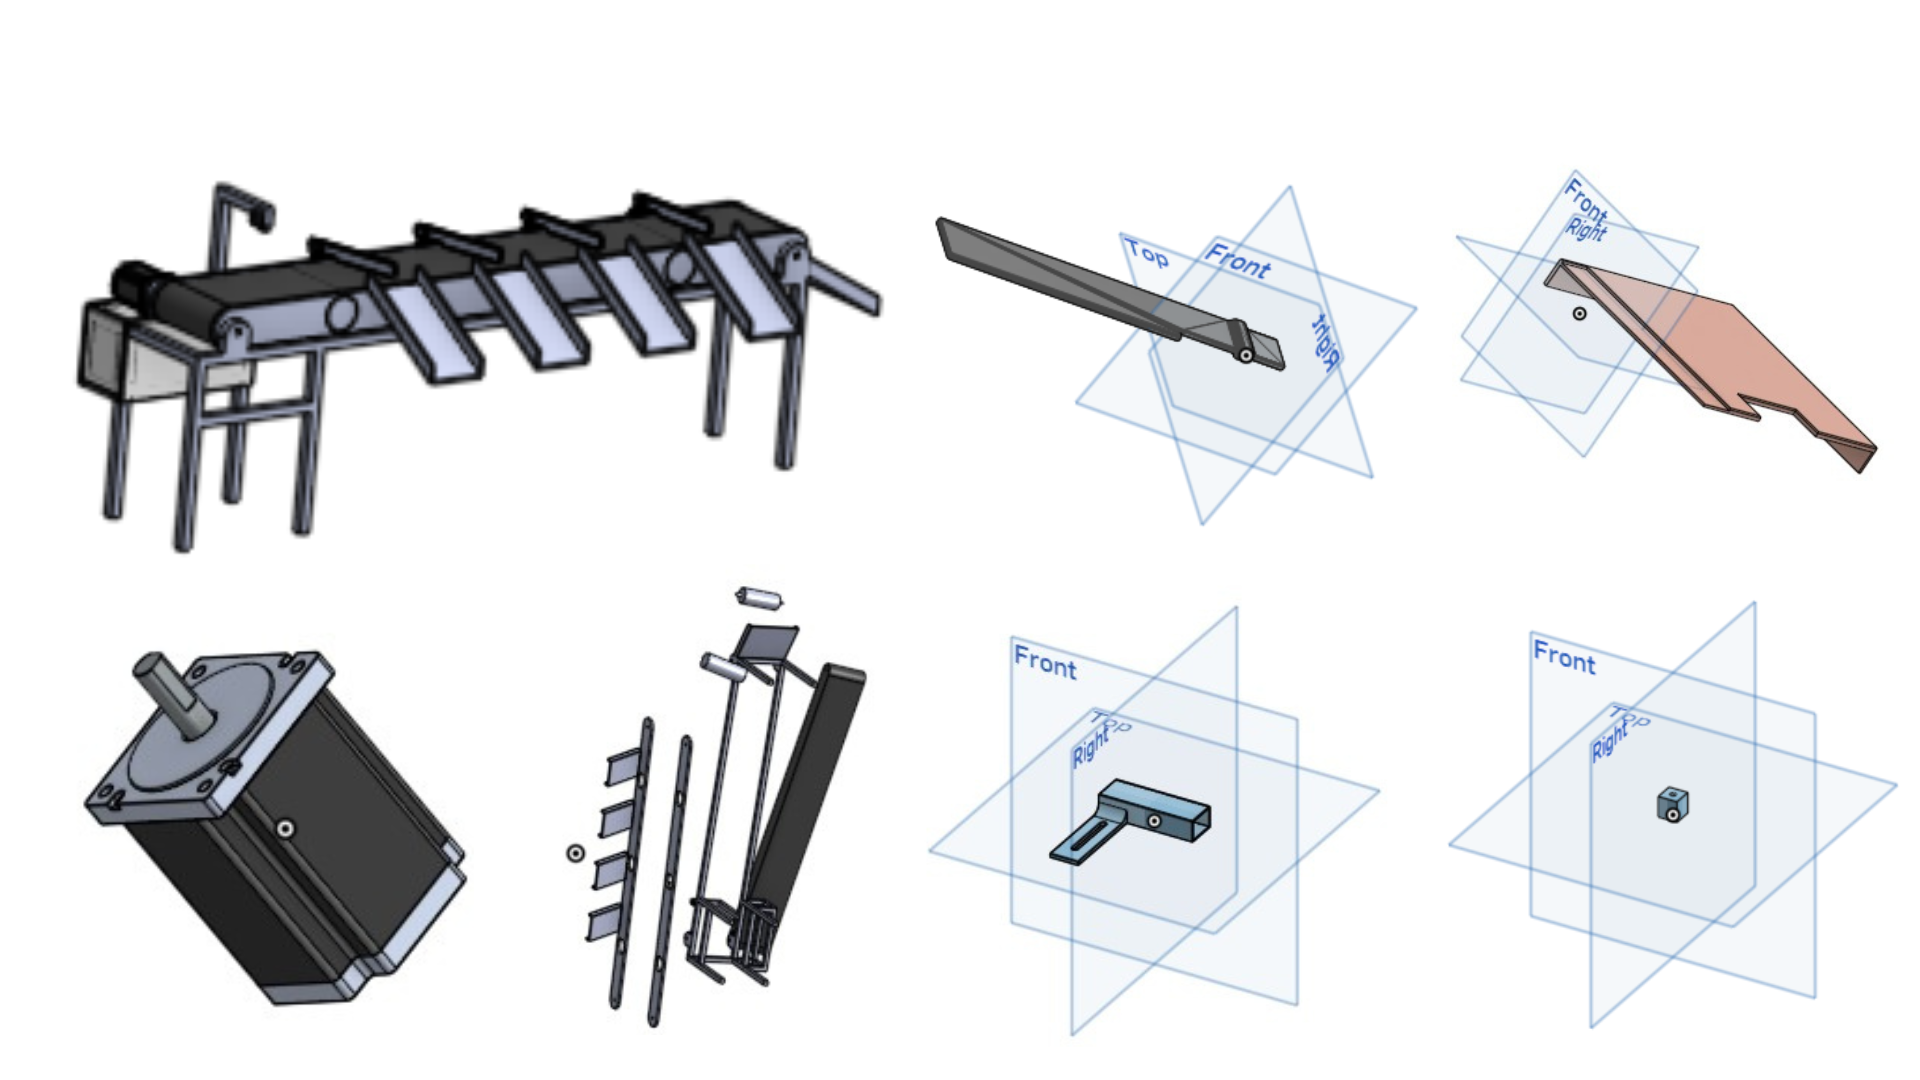
\includegraphics[width=0.9\linewidth]{figures/CAD.png}
\caption{Computer aided design model and assembled hardware prototype}
\label{fig:prototype}
\end{figure}

\subsection{Software System Development}
\label{sec:m_softwaredev}

The software consists of a Python application centered on a web-based operator dashboard, supported by a detection module and a local database. The dashboard displays a live camera feed overlaid with bounding boxes. It also presents the current tracking status, the most recent fruit's class and confidence score, and an indicator panel showing total fruits processed, throughput, defect ratio, and average shelf life over a specified time window. Additionally, it includes a class-distribution chart and a tabular log of recent detections.

The model is loaded once per session. A menu allows the operator to select between trained checkpoints, and every frame is processed at an adjustable confidence threshold (defaulting to 0.45). Every finalized classification is saved to the database along with its confidence score, bounding box coordinates, timestamp, and shelf-life value. Because the indicator panel reads directly from this database, the displayed dashboard metrics consistently reflect the stored data.

\begin{figure}[H]
\centering
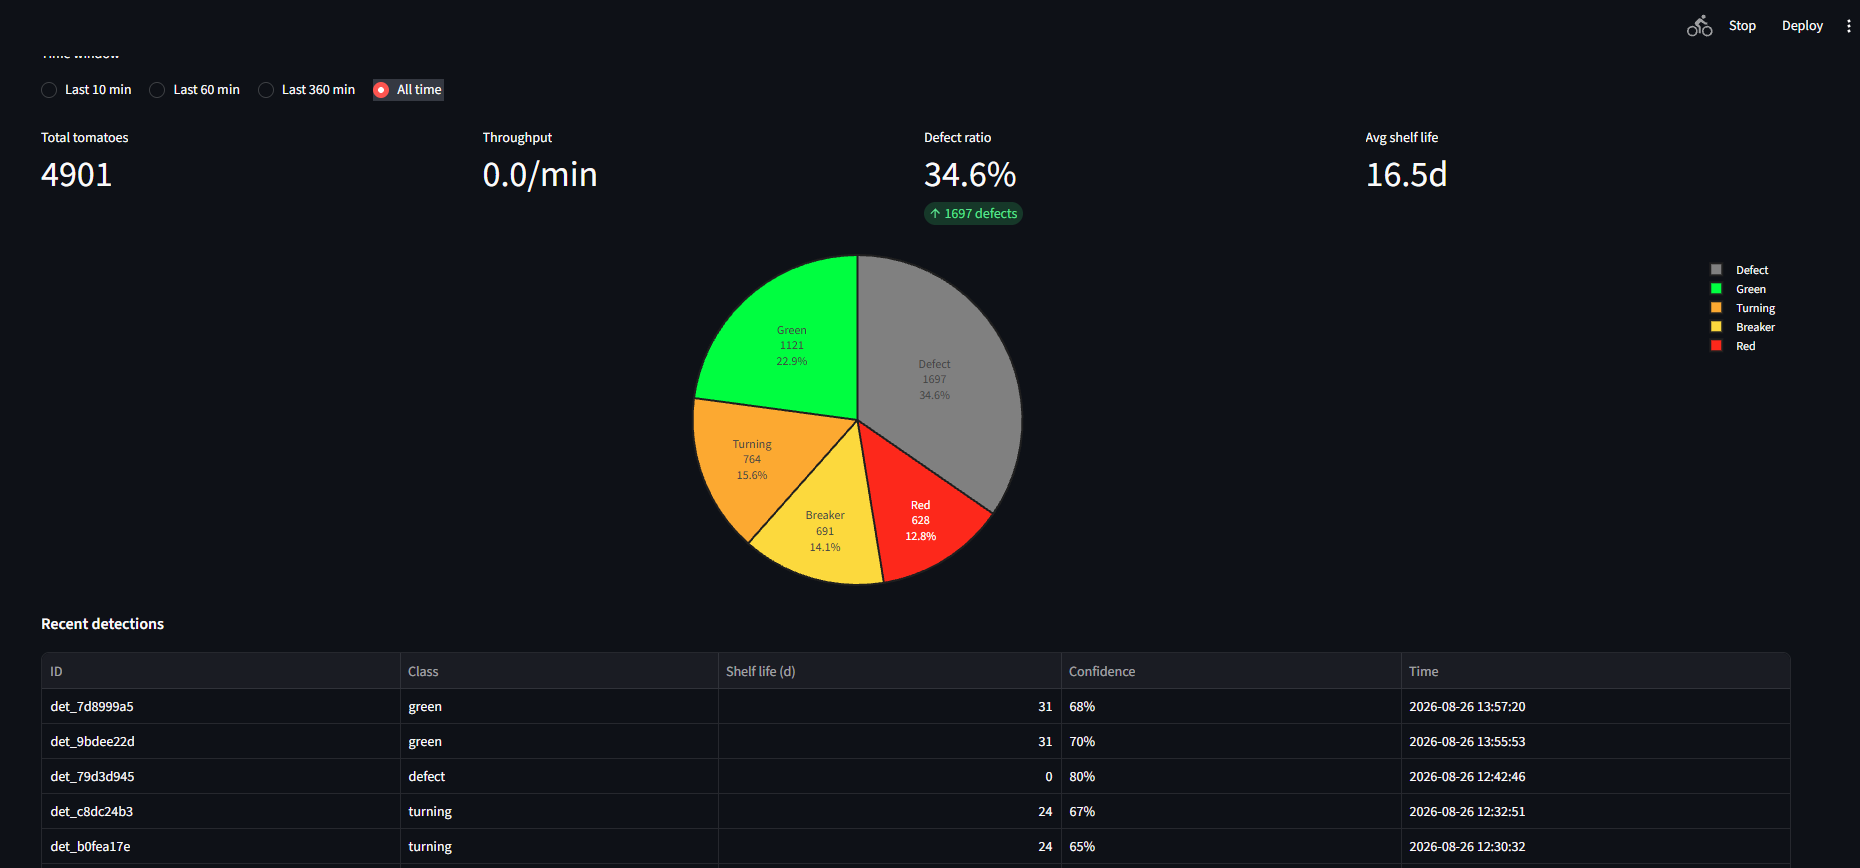
\includegraphics[width=0.9\linewidth]{figures/Dashboard.png}
\caption{Software architecture and operator dashboard of the detection and sorting application}
\label{fig:software}
\end{figure}

\subsection{Hardware and Software Integration}
\label{sec:m_integration}

The dashboard communicates with the microcontroller via Bluetooth. Upon classification, the host computer sends a brief command indicating either one of the four gate assignments or a no-gate assignment for a defective fruit. Each command includes a sequence number and is repeatedly transmitted until acknowledged, up to a defined retry limit. If the microcontroller receives a command it has already executed, it acknowledges the command again but does not duplicate the physical action. Both mechanisms are crucial: a lost command removes a fruit from the sorting queue, while a missing acknowledgment duplicates it. Either error would disrupt all subsequent gate assignments.

Within the microcontroller, each gate maintains an independent queue of pending classifications, ordered identically to how the fruits travel along the belt. When a gate's sensor detects an approaching fruit, the system evaluates the item at the front of that specific gate's queue. If the classification matches the gate's designated class, the gate actuates. If it does not match, the item is transferred to the subsequent gate's queue for future evaluation. This logic ensures that every classification remains synchronized with the physical fruit it represents, even when multiple fruits are simultaneously moving on the belt.

Each gate is triggered by its own presence sensor rather than relying on a time delay calculated from belt speed and distance. This approach eliminates the primary source of timing error, which typically worsens for gates located further down the conveyor belt. A brief delay, dynamically scaled to the belt speed, compensates for the physical gap between the sensor and the diverter blade. The gate then remains open momentarily before returning to its resting state.

\subsection{Shelf Life Observation Procedure}
\label{sec:m_shelflife}

Shelf life was measured observationally rather than predicted by a mathematical model. A total of 50 green \textit{Padma} tomatoes of known starting stages were maintained at ambient room temperature and observed over a continuous 31-day period. Every morning between 7:00 and 7:20 a.m., each fruit was photographed from four angles. Color differentiation was utilized to categorize the fruit into one of the four stages detailed in Table~\ref{tab:ripeness}, and the duration spent in each stage was recorded. A fruit was removed from the study once it became unmarketable specifically when it became noticeably soft, molded, rotting, or severely blemished.

The estimated remaining shelf life for a detected class is calculated as the remaining time in that current stage plus the full duration of all subsequent stages. For instance, a fruit detected as a breaker is credited with the remaining breaker stage duration plus the complete duration of the turning and red stages. This represents an upper bound rather than an exact value, because a single static image cannot determine how long a fruit has already been in its current stage. A fruit classified as defective is assigned a shelf life of zero, as it is rejected at the sorting point. These per-class values are stored in a fixed lookup table and applied instantly upon classification. The comprehensive observation records are available in \hyperref[app:B]{Appendix~B}.

\subsection{Complete End to End System Process}
\label{sec:m_endtoend}

The process begins with fruit collection, pre-sorting, and photography under controlled lighting. The images are then annotated, preprocessed, augmented, and divided into three dataset splits; the detector is trained and evaluated using these sets. During deployment, each live frame is processed through the trained model. Each fruit is tracked and classified according to the methodology in Section~\ref{sec:m_realtime}. The final classification generates a sorting command, the corresponding gate actuates when the fruit triggers its sensor, and the classification, confidence score, and estimated shelf life are subsequently logged and displayed on the dashboard.

\begin{figure}[H]
\centering
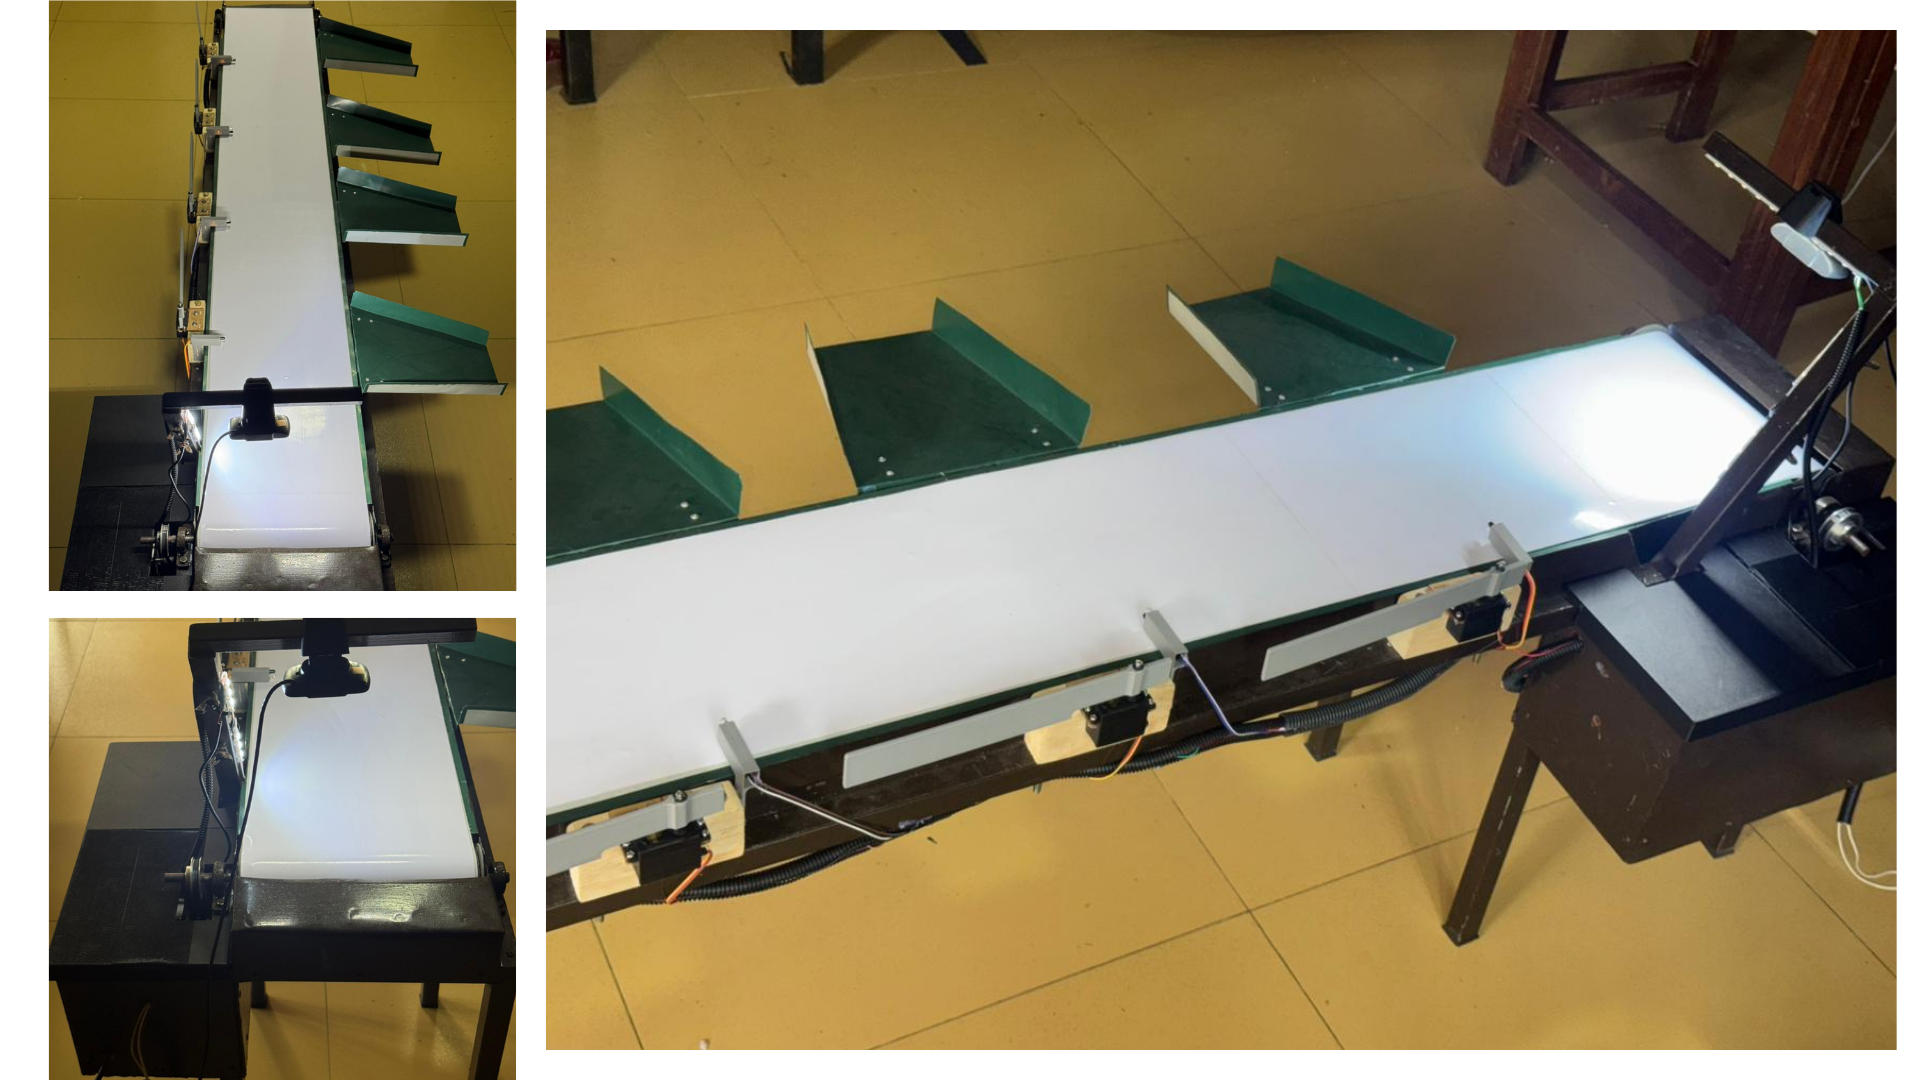
\includegraphics[width=0.9\linewidth]{figures/Untitled design (2).png}
\caption{Complete end to end system workflow}
\label{fig:workflow}
\end{figure}

\subsection{Experimental Procedure}
\label{sec:m_experiments}

Five experiments were conducted to evaluate the system.

\textbf{Experiment 1 -- Held-out test evaluation.} Evaluates detection and classification performance on unseen data using the dataset from Section~\ref{sec:m_dataset} and the procedures from Sections~\ref{sec:m_training} and~\ref{sec:m_evaluation}. Metrics include precision, recall, mAP@50, and mAP@50--95, both per class and overall, derived from a single evaluation pass over the fixed test set.

\textbf{Experiment 2 -- Architecture comparison.} Compares the deployed YOLOv8m model against a YOLO26m model trained and tested on the same dataset. This ensures the chosen architecture is supported by experimental evidence from this project. The two training sessions were not identical one utilized a fixed batch size while the other used automatic batch selection, and they terminated after different numbers of epochs. These methodological differences are explicitly reported alongside the results.

\textbf{Experiment 3 -- Live classification validation.} Verifies classification accuracy outside the offline test set by presenting fruits of known classes to the live camera inside the lightbox and recording the dashboard's output. This experiment originally identified the lighting inconsistency discussed in Section~\ref{sec:annotation_qc}, and was repeated after the issue was resolved. The recorded metric is the proportion of fruits correctly classified.

\textbf{Experiment 4 -- Conveyor transport and end-to-end sorting.} Evaluates the conveyor system using fruit of known classes placed on the belt. This experiment consists of two phases: a mechanical trial with inactive cameras and sorting logic to verify smooth and stable transport, and a fully operational trial to measure the frequency of correct gate diversions.

\textbf{Experiment 5 -- Shelf-life observation.} Conducts the observational study detailed in Section~\ref{sec:m_shelflife} to document the duration each fruit spends in each ripening stage.

Raw records for all five experiments are given in \hyperref[app:B]{Appendix~B}.

\subsection{System Testing Procedure}
\label{sec:m_testing}

System testing was structured into four phases: controlled testing under lightbox illumination; stress testing involving variations in fruit orientation, occlusion, distance, and lighting; testing under realistic operational conditions; and comparing automated grading against manual grading. The corresponding test cases are outlined in Table~\ref{tab:testcases}, and the outcomes, including pass/fail statuses, are reported in Chapter~\ref{ch:results}.

\begin{table}[H]
\caption{System test cases and expected results}
\label{tab:testcases}
\centering
\begin{tabularx}{\textwidth}{l p{4.0cm} p{3.2cm} X}
\toprule
\textbf{ID} & \textbf{Test description} & \textbf{Input} & \textbf{Expected result} \\
\midrule
T-01 & Held-out test set detection and classification accuracy & 777 unseen labelled images & High precision, recall and mean average precision across all five classes \\
T-02 & Architecture comparison on the same held-out split & Two trained checkpoints & A defensible basis for the deployed architecture choice \\
T-03 & Live classification inside the lightbox & Known-class fruit, live camera & Correct class reported for each fruit presented \\
T-04 & Conveyor belt mechanical transport & Fresh fruit on the running belt & Smooth and stable transport without stalling or displacement \\
T-05 & Non-tomato object rejection & Frame containing fruit and distractor objects & Distractors not classified into any tomato class \\
T-06 & Single gate actuation bench test & Direct command to one gate, belt stationary & Corresponding servo opens and returns automatically \\
T-07 & End-to-end sorting accuracy & Known-class fruit moving on the running belt & Fruit physically diverted at the correct gate \\
T-08 & Wireless command reliability under retry & Sequenced class commands over the live link & Commands delivered exactly once despite intermittent packet loss \\
\bottomrule
\end{tabularx}
\end{table}

These cases cover detection accuracy (T-01, T-02), classification (T-03), mechanical function (T-04, T-06), and integration (T-05, T-07, T-08).

\subsection{Ethical and Safety Considerations}
\label{sec:m_ethics}

This research focused exclusively on food produce and a prototype conveyor system. Because it did not involve human or animal subjects, nor the collection of personal data, an ethics board review was not required. Given the 24\,V and 12\,V power supplies, wiring was inspected before every powered test. The conveyor belt, rollers, motor, and gate servos present pinch-point hazards; therefore, the belt area was kept clear of hands during operation. Fruit utilized for photography and conveyor testing was handled and disposed of hygienically. No destructive testing was performed, aside from the shelf-life study, during which the fruit naturally spoiled by design. Finally, images initially sourced from a public dataset were utilized in accordance with the dataset's licensing terms and were subsequently removed from the final dataset, as detailed in Section~\ref{sec:annotation_qc}.

\clearpage